\chapter{第一个程序}
\label{ch:01}

ChaLi 是哪五个字母 —— 每个字母锁一条契约，记住了后面每章都能对上号：

{\small\setlength{\tabcolsep}{4pt}
\begin{longtable}{>{\raggedright\arraybackslash}p{\dimexpr 0.048\linewidth-2\tabcolsep\relax}>{\raggedright\arraybackslash}p{\dimexpr 0.314\linewidth-2\tabcolsep\relax}>{\raggedright\arraybackslash}p{\dimexpr 0.618\linewidth-2\tabcolsep\relax}}
\toprule
字母 & 含义 & 契约 \\
\midrule
\endhead
C & Copy（深拷贝值语义） & 赋值就是彻底的复制，绝不共享内存。大对象必须显式用引用传。 \\
H & Hygienic（卫生宏） & 在编译期做安全的代码替换，绝不意外捕获或污染外部变量。 \\
A & Any（万能盒子 / 类型擦除） & 没有泛型约束时，可以装下任何类型的数据。 \\
L & Lifetime（生命周期 / 借用检查器） & 引用永远不能活得比它的数据源更久，否则编译直接报错（\texttt{CHL1204}）。 \\
I & Interface（接口 / 运行期多态） & 定义一组共同的“契约”，运行期根据对象的实际类型进行分派。 \\
\bottomrule
\end{longtable}
}

万事开头难，但这一章只干三件事：把工具装好、跑出一行字、看懂这行字是怎么来的。

读完这一章，你会有第一个能跑的程序，也会知道「出错」在 ChaLi 里长什么样——后者比前者重要，因为接下来每一章你都会用到它。

\section{把工具装好}

ChaLi 只有一个命令行程序，叫 \texttt{chali}，编译、建工程、跑测试全在它里面。装它有两条路。

这条路最短：用安装包。 Windows 使用 MSI，Ubuntu/Debian 使用 DEB，CentOS 使用 RPM；安装后通过 PATH 中的 \texttt{chali} 命令启动。包名、架构及手动安装方法见\href{https://github.com/rabbitc999/ChaLi/blob/master/doc/42-installation-packages.md}{安装与多架构构建}。

这条路最全：从源码构建。 适合想改编译器的人，也适合想看清内部的人：

\par
\medskip
\begin{lstlisting}[style=sh]
sh gen.sh      # 用 IELR 从 chali.gram 生成前端
make           # 按当前平台与 LLVM 配置生成编译器和静态库
\end{lstlisting}
\par
\medskip

\texttt{gen.\allowbreak{}sh} 需要一份 \href{https://github.com/rabbitc999/ParseEngine}{ParseEngine} 文法生成器，细节见\href{https://github.com/rabbitc999/ChaLi/blob/master/doc/01-quickstart.md#1-安装}{快速开始}，这里不展开。

装完了，敲一句：

\par
\medskip
\begin{lstlisting}[style=sh]
chali help
\end{lstlisting}
\par
\medskip

屏幕上滚出一大串用法，就说明装好了。先别急着读完那串帮助——那是给有经验的人查的，跟着这本书走，你会一个个认识里面的选项。

\begin{tip}{Windows 用户注意}
MSI 安装后的命令是 \texttt{chali}；源码默认构建的外置 LLVM 文件名为\texttt{chali-1.\allowbreak{}0.\allowbreak{}8-llvm-external-windows-x64.\allowbreak{}exe}，可在 PowerShell 中用\texttt{.\allowbreak{}/\allowbreak{}chali-1.\allowbreak{}0.\allowbreak{}8-llvm-external-windows-x64.\allowbreak{}exe help} 启动。静态变体使用 \texttt{llvm-static}。本书的 \texttt{chali} 命令默认指已安装到 PATH 的编译器；直接运行构建产物时，请换成实际文件路径。
\end{tip}

\section{Hello, ChaLi}

新建一个文件 \texttt{hello.\allowbreak{}chl}，内容如下：

\par
\medskip
\begin{lstlisting}[style=chali]
void main()
{
    println("Hello, ChaLi!");
}
\end{lstlisting}
\par
\medskip

\par
\medskip
\begin{lstlisting}[style=out]
Hello, ChaLi!
\end{lstlisting}
\par
\medskip

然后运行它：

\par
\medskip
\begin{lstlisting}[style=sh]
chali run hello.chl
\end{lstlisting}
\par
\medskip

屏幕上出现 \texttt{Hello,\allowbreak{} Cha\allowbreak{}Li!}，第一个程序就成了。

\texttt{chali run} 这个写法看着啰嗦，其实 \texttt{run} 是可以省的——直接

\par
\medskip
\begin{lstlisting}[style=sh]
chali hello.chl
\end{lstlisting}
\par
\medskip

效果一样。但本书会一直写 \texttt{chali run}，因为把场景写出来在人多的时候少很多误会：\texttt{chali hello.\allowbreak{}chl Alice} 和 \texttt{chali run hello.\allowbreak{}chl Alice} 是同一件事，但 \texttt{chali check hello.\allowbreak{}chl} 完全是另一件事。

\section{逐行看懂它}

就三行，一行一行来。

第一行：\texttt{void main(\allowbreak{})\allowbreak{} \{}

程序从哪里开始跑？从 \texttt{main} 开始。这个名字是定死的，不能改成 \texttt{Main}、\texttt{start} 或者别的什么。前面的 \texttt{void} 是它返回的东西的类型，\texttt{(\allowbreak{})\allowbreak{}} 里现在空着，意思是它不接收参数。

第二行：\texttt{println(\allowbreak{}"Hello,\allowbreak{} Cha\allowbreak{}Li!")\allowbreak{};}

\texttt{println} 是「打印一行」的意思：把括号里的东西写到屏幕上，末尾自动换行。它是 ChaLi 核心库里最常用的函数，不用 \texttt{import} 就能用。

行尾那个 \texttt{;} 是分号，表示这句话说完了。跟 C、Java 一样。

最后的花括号 \texttt{\}} 是 \texttt{main} 的结尾。

看出来了吗——花括号划范围，分号断句，这和 C 系语言一模一样。这是 ChaLi 刻意这么做的：你已经会的东西，它不想让你重学一遍。

\section{\texttt{run} 和 \texttt{check}}

现在故意把程序弄坏一次，看看会发生什么。把第二行末尾的分号删掉：

\par
\medskip
\begin{lstlisting}[style=chali]
void main()
{
    int64 x = 1
}
\end{lstlisting}
\par
\medskip

再跑后，诊断会指向缺少分号之后的记号。源码摘录如下（诊断候选列表以实际编译器输出为准）：

\par
\medskip
\begin{lstlisting}[style=out]
 3 |     int64 x = 1
 4 | }
\end{lstlisting}
\par
\medskip

三件事值得注意：

\begin{itemize}

\item 它给出文件名、行列位置和相关源码；定位可能落在后面的右花括号上。第 3 行少了个分号，解析器读完声明后仍在等待分号，遇到 \texttt{\}} 才确认无法继续。看到报错位置和你以为的不一致时，先看报错位置的前面。

\item 内部记号名被翻译成了人话，例如 \texttt{条件(\allowbreak{}if)\allowbreak{}}。默认中文环境下可以直接阅读。报错语言跟着系统走，可以用 \texttt{chali lang en} 或环境变量 \texttt{CHALI\_LANG} 换掉。

\item 候选列表说明它正在等待什么。这种话现在看不懂没关系，以后你写多了，一眼就知道是「这里少了个东西」。

\end{itemize}

重要：这个错误是编译期就报出来的，程序一个字符都没执行。这就是 ChaLi 和其他很多语言不同的地方——能编译期拦住的，绝不放到运行期。

如果你只想检查代码写没写对、不想真的跑它，用：

\par
\medskip
\begin{lstlisting}[style=sh]
chali check hello.chl
\end{lstlisting}
\par
\medskip

\texttt{check} 做前两步（预处理、解析与类型检查），不执行、也不产出文件。写代码的时候这个命令用得比 \texttt{run} 还多：先 check 再 run，能省掉很多「跑到一半才发现写错了」的时间。

\begin{tip}{提示}
还有个更细的用法：\texttt{chali check hello.\allowbreak{}chl json}，输出机器可读的 JSON 诊断。这是给编辑器插件用的，平时不用管。
\end{tip}

\section{那行字背后发生了什么}

\texttt{chali run} 看着像「执行脚本」，其实它在一个进程里做完了四件事：

\begin{enumerate}

\item 预处理 —— 处理 \texttt{\%define}、\texttt{\%if} 这类指令（第 19 章讲）；

\item 解析与类型检查 —— 语法、类型、引用的生命周期都在这里查，不通过就不执行；

\item 生成并优化四元式 —— 把程序翻译成四元式 IR，按完整优化预算化简；

\item AOT 编译执行 —— 经 LLVM 生成原生机器码，在当前进程里跑起来。

\end{enumerate}

前三步是「编译」，第四步生成机器码后执行。把 \texttt{run} 换成别的场景词，前三步是一样的，只是最后一步换了形态：

\begin{center}
\begin{tabular}{ll}
\toprule
你想 & 命令 \\
\midrule
直接跑起来 & \texttt{chali run src/\allowbreak{}main.\allowbreak{}chl} \\
只检查、不跑 & \texttt{chali check src/\allowbreak{}main.\allowbreak{}chl} \\
\bottomrule
\end{tabular}
\end{center}

这两条路的区别在第 22 章讲；现在你只要知道：同一份源码，可以有好几种走法。

\section{从源码到原生程序：编译流程图}

编译流程如下。条件预处理决定哪些代码参与编译；文法生成的词法与语法前端建立 AST，宏模板也在其中。卫生宏在语义分析时展开，并与类型推导配合，之后完成名称、类型、泛型和借用检查。

\begin{center}
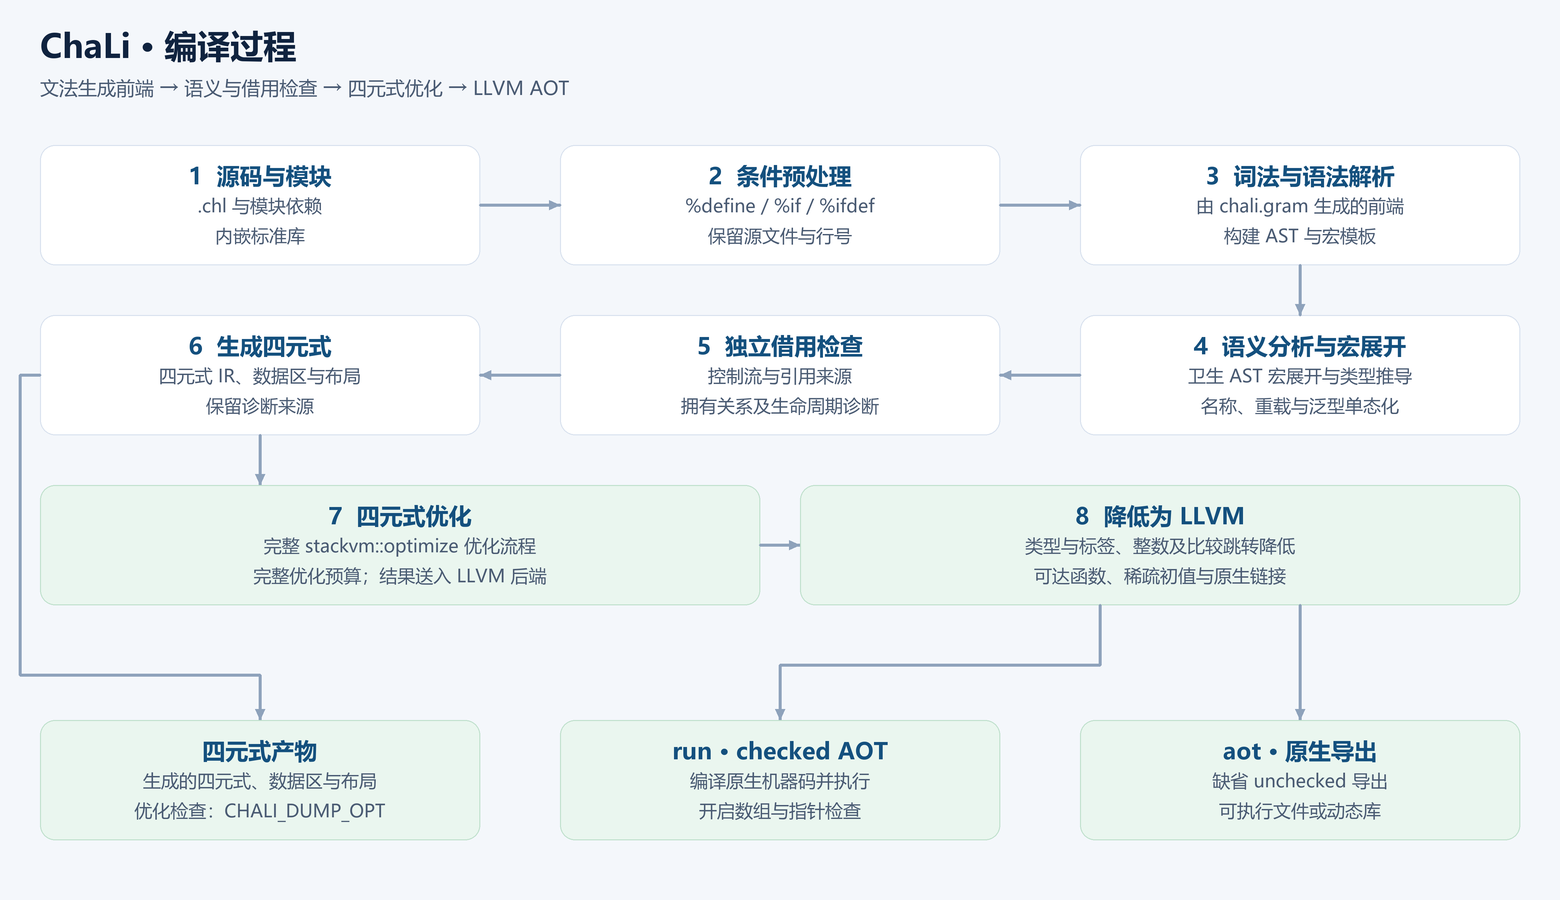
\includegraphics[width=\linewidth]{../images/chali-compilation.png}\par
ChaLi 编译流程：预处理、解析、语义期宏展开、借用检查、四元式优化与 LLVM AOT
\end{center}

四元式是本书所说的 IR。编译器生成四元式、数据区和布局，执行路径对四元式完成完整优化后送入 LLVM 后端，生成原生机器码；优化结果可通过调试输出检查，与生成阶段的四元式产物出口不要混淆。

\texttt{run} 与 \texttt{aot} 都产出原生程序：\texttt{run} 走 checked AOT 编译并当场执行，\texttt{aot} 默认 unchecked 导出可执行文件或动态库；部署边界见第 22 章，AOT 导出见第 25 章。

图与仓库 README 使用相同绘图脚本生成。内嵌手册导出时携带图片，PDF 也直接收录图片，所以离线阅读不依赖网络。

\section{小结}

这一章你认识了：

\begin{itemize}

\item 入口函数固定叫 \texttt{main}，返回 \texttt{void}；\texttt{void main} 正常完成时退出码为 0，panic 仍失败；

\item \texttt{println(\allowbreak{}.\allowbreak{}.\allowbreak{}.\allowbreak{})\allowbreak{}} 打印一行，来自核心库，不用 import；

\item 分号断句、花括号划范围，和 C 系语言一样；

\item \texttt{chali run} 跑，\texttt{chali check} 只查；

\item 报错会给出行列位置和画了波浪线的源码，而且大多在编译期就报出来了。

\end{itemize}

还有一件事本章没讲：\texttt{println} 为什么不用 \texttt{import}？因为它属于核心模块 \texttt{lang}，而 \texttt{lang} 是自动加载的。别的模块就没这个待遇了，第 18 章会讲清楚。

\section{下一步}

光看「Hello, ChaLi」是学不会编程的。下一章我们写一个真的有用的小程序：键盘猜数字。它会用到变量、输入、循环和分支——四个最基础的积木，而且你会看到它们是怎么串在一起的。

翻到\hyperref[ch:02]{第 2 章 猜数字}。

\section{边界与验证}

通过语法和类型检查，只能证明对应静态检查通过。程序是否产生预期输出、是否访问了外部资源，需要运行验证；外部输入变化也可能使后续运行失败。

\section{习题}

前两题用于理解和基本实现，第三题检查边界，最后一题为综合挑战。先独立完成，再核对参考解答。

\begin{enumerate}

\item 解释检查成功与运行结果正确之间的区别。

\item 把欢迎程序改为输出两行，分别为自己的名字和 Hello, ChaLi!。

\item 删掉语句末尾的分号，检查诊断位置，再修复。

\item 挑战：写出一个检查成功、运行时断言失败的完整程序。

\end{enumerate}

\subsection*{参考解答与验收要点}

\begin{enumerate}

\item 检查不执行全部业务路径；运行时还可能发生断言、输入或宿主错误。至少分别记录检查状态、退出状态和实际输出。

\item 使用两次 println，逐行对照输出；不要把编辑器显示的文字当成程序输出。

\item 这是语法错误练习，应在检查阶段失败。记录文件、行列和具体缺失内容，不把整条诊断文案写死。

\item 在 main 内调用 assert(false)，检查成功但执行失败；将它作为故意失败用例单独保存。

\end{enumerate}

\section{番外：皇帝的新程序}

改写自安徒生《皇帝的新装》。

许多年以前，有一位皇帝，为了运行得漂亮，不惜把所有的钱都花在买新程序上。他既不关心输入，也不关心输出，除非是为了炫耀他的新基准。他每一天钟头都要换一套编译选项。人们提到他，总是说：“皇上在优化器里。”

有一天来了两个骗子，自称能编出人类所能想象的最快程序。这程序还有一种奇怪的特性：凡是不称职或愚蠢得不可救药的人，都看不见它的输出。

“这正是我理想中的程序！”皇帝想，“有了它，我就能知道群臣里谁不懂技术。”于是付了许多预算，叫他们立刻开工。骗子架起两台显示器，整日敲空格；最好的服务器和显卡，却都装进了自己的口袋。

老大臣奉命去看，睁大眼睛，只见 \texttt{void main(\allowbreak{})\allowbreak{} \{\}}。他不敢说自己什么也没看见，便连连点头：“多么优美的输出！多么鲜艳的性能！”骗子请他描述结果，他说：“非常符合预期。”因为预期也没有写。

游行那天，皇帝举着空屏幕，内臣托着并不存在的进度条。百姓齐声称赞：“运行得真快！连日志也没有！”谁也不愿显得自己不称职。

“可是它什么也没做呀！”一个孩子终于叫了出来。

皇帝有点发抖，因为他觉得孩子说的似乎是对的。他心里却想：“这发布会必须坚持到底。”于是更加骄傲地举着屏幕，内臣们继续托着那根根本不存在的进度条。

\subsection*{技术对照}

通过语法和类型检查，只能证明对应静态检查通过。程序是否产生预期输出、是否访问了外部资源，需要运行验证；外部输入变化也可能使后续运行失败。
